\subsection{Autenticazione} 
\subsubsection{Registrazione}

\begin{figure}[!h]
	\centering
	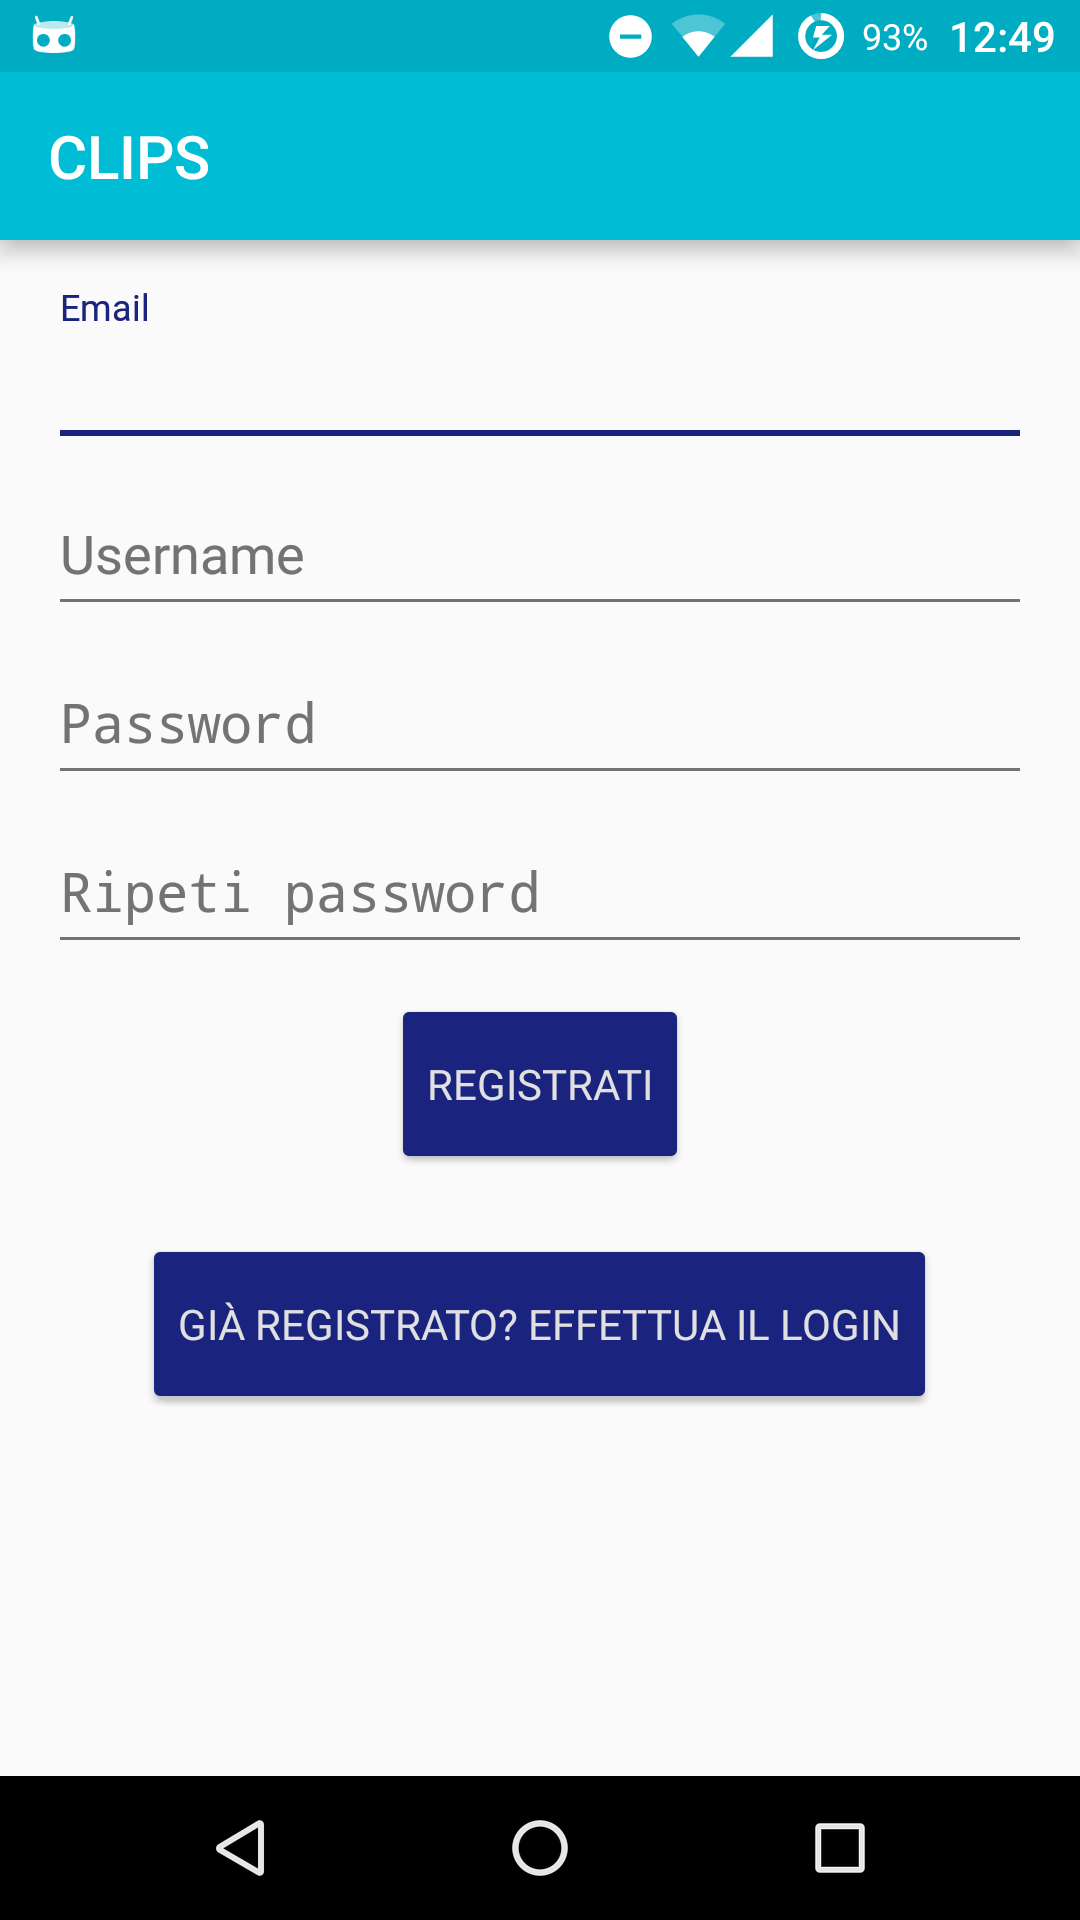
\includegraphics[scale=0.15]{screenshot/Registrazione}
	\caption{Schermata di registrazione}
\end{figure}

Attraverso questa schermata l'utente deve inserire nella form tutti i dati richiesti e successivamente potrà registrarsi cliccando l'apposito bottone ``REGISTRATI''. Successivamente verrà automaticamente autenticato nel sistema.
Se l'utente invece si fosse già registrato nel sistema precedentemente potrà accedere alla schermata di Login tramite il bottone ``GIÀ REGISTRATO? EFFETTUA IL LOGIN'', oppure tramite l'apposito elemento nel menu.
\newpage

\subsubsection{Login}
\begin{figure}[!h]
	\centering
	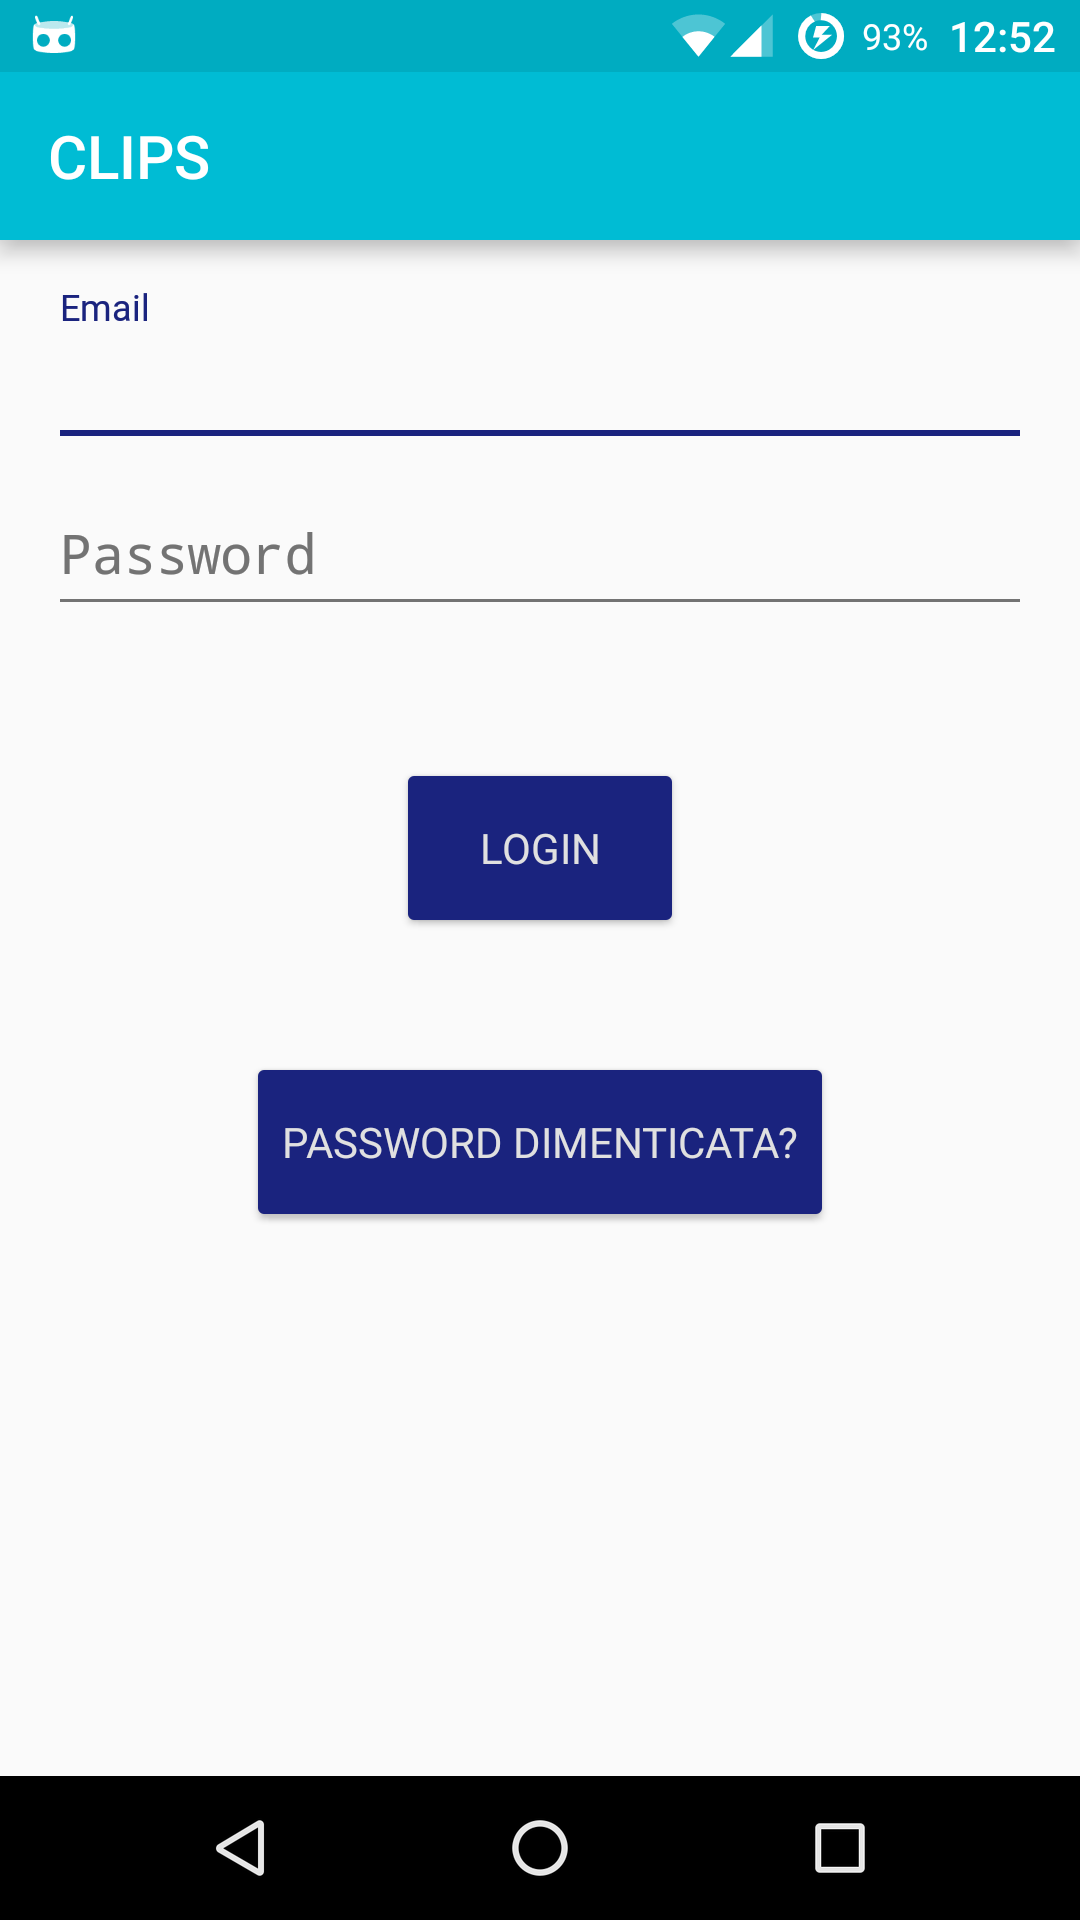
\includegraphics[scale=0.15]{screenshot/login}
	\caption{Schermata di registrazione}
\end{figure}
Qualora un utente si fosse già registrato nel sistema può accedere a questa schermata che gli consentirà, inserendo Email e Password di accedere al sistema.
\newpage


\subsubsection{Account}
\begin{figure}[!h]
	\centering
	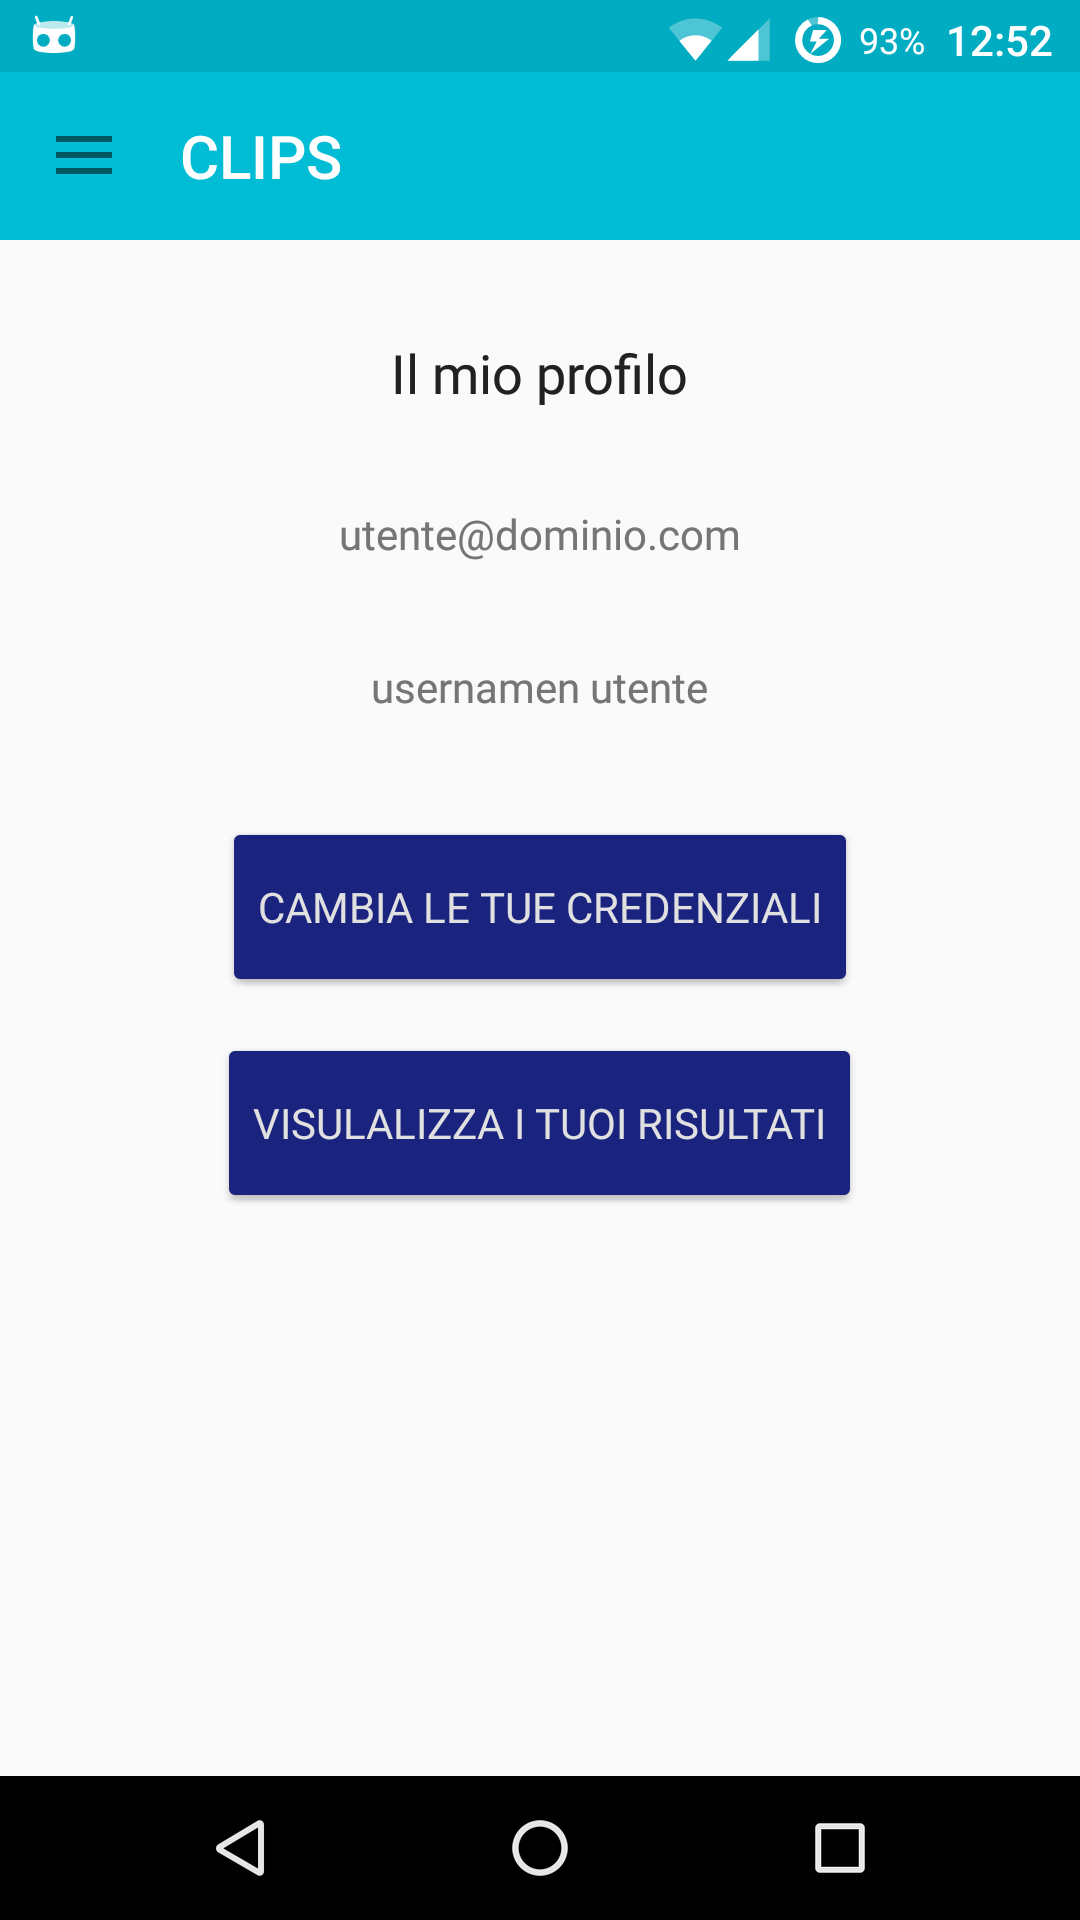
\includegraphics[scale=0.15]{screenshot/account}
	\caption{Schermata di registrazione}
\end{figure}
In questa schermata è possibile vedere i propri dati di registrazione. Sono presenti anche due bottoni: ``CAMBIA LE TUE CREDENZIALI'' indirizza l'utente in una pagina da cui potrà cambiare il proprio username e la propria password, ``VISUALIZZA I TUOI RISULTATI'' indirizza ad una schermata in cui l'utente può visualizzare i propri risultati